\subsection{Casi d'Uso}

    \begin{figure}[h]
        \centering
        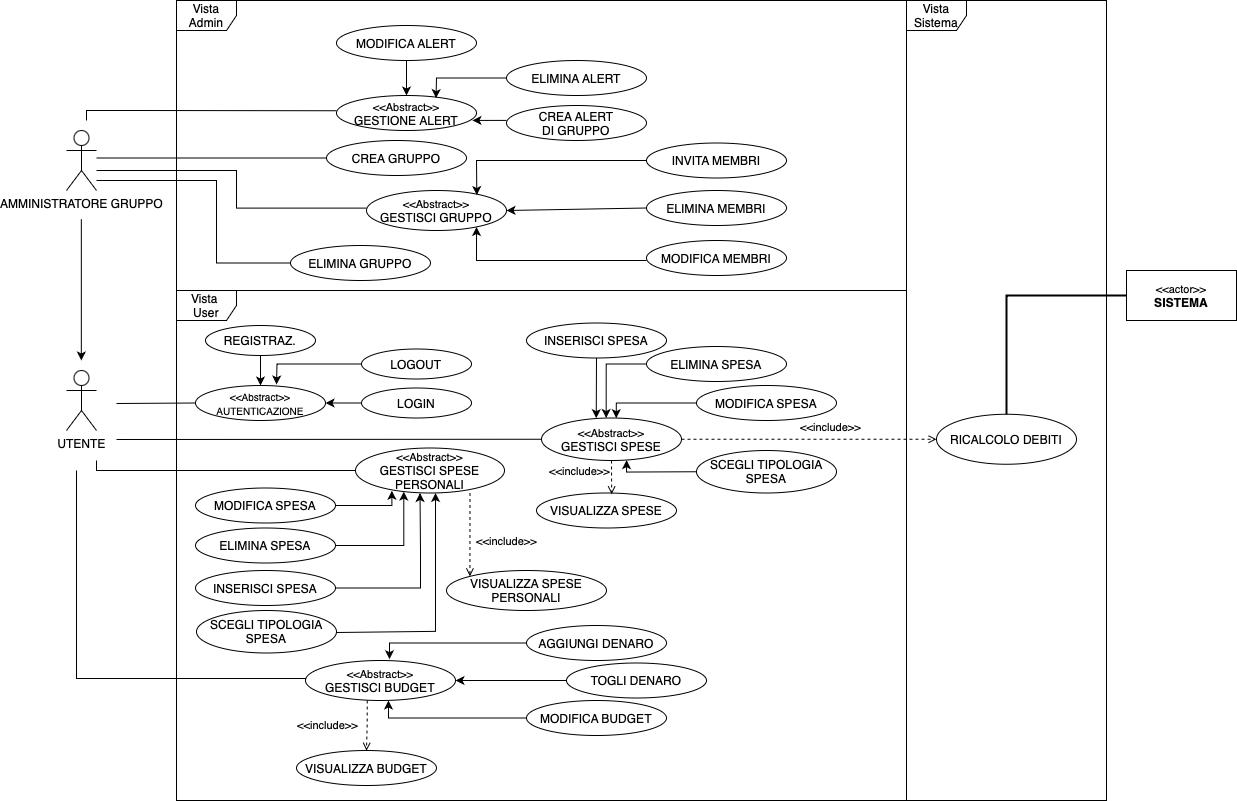
\includegraphics[width=1.1\textwidth, trim=3cm 0cm 1cm 0cm]{images/DiagrammaCasiDusoV1.2.png}
        \caption{Diagramma casi d'uso }
    \end{figure}

Di seguito sono riportati i casi d'uso in figura:
\begin{itemize}
    \item \textbf{UC1 - Login}: Come utente, voglio poter accedere al mio account per gestire le mie spese.
    \item \textbf{UC2 - Registrazione}: Come nuovo utente, voglio potermi registrare al sistema per iniziare a usare la web-app.
    \item \textbf{UC3 - Logout}: Voglio poter terminare la mia sessione.
    \item \textbf{UC4 - Crea alert di gruppo}: Come utente amministratore di un gruppo spesa voglio poter inserire un alert, dove un alert è un avviso che ci permette di avvisare se si sta raggiungendo una soglia limite di spesa.
    \item \textbf{UC5 - Modifica alert}: Voglio poter modificare i valori dell'alert.
    \item \textbf{UC6 - Elimina alert}: Voglio poter eliminare l'alert. 
    \item \textbf{UC7 - Crea gruppo}: Voglio poter creare un gruppo di condivisione spese. 
    \item \textbf{UC8 - Invita memebri}: Voglio come amministratore invitare membri nel gruppo di spese.
    \item \textbf{UC9 - Elimina membri}: Voglio come amministratore poter eliminare membri del gruppo di spese.
    \item \textbf{UC10 - Modifica membri}: Voglio come amministratore modificare i membri nel gruppo di spese.
    \item \textbf{UC11 - Elimina gruppo}: Voglio poter eliminare un gruppo di condivisione spese. 
    \item \textbf{UC12 - Accedi gruppo}: Voglio poter accedere ad un gruppo di condivisione spese. 
    \item \textbf{UC13 - Inserisci spesa}: Voglio poter inserire una spesa di gruppo.
    \item \textbf{UC14 - Elimina spesa}: Voglio poter eliminare una spesa di gruppo.
    \item \textbf{UC15 - Modifica spesa}: Voglio poter modificare una spesa di gruppo.
    \item \textbf{UC16 - scegli tipologia spesa}: Voglio poter scegliere la tipologia di spesa.
    \item \textbf{UC17- Visualizza spese}: Voglio poter visualizzare le spesa di gruppo.
    \item \textbf{UC18 - Ricalcolo debiti}: Voglio poter calcolare i debiti.
    \item \textbf{UC19 - Inserisci spesa personale}: Voglio poter inserire una spesa personali.
    \item \textbf{UC20 - Elimina spesa personale}: Voglio poter eliminare una spesa personali.
    \item \textbf{UC21 - Modifica spesa personale}: Voglio poter modificare una spesa personali.
    \item \textbf{UC22 - scegli tipologia spesa personale}: Voglio poter scegliere la tipologia di spesa personale.
    \item \textbf{UC23 - Visualizza spesa personale}: Voglio poter visualizzare le spesa personali.
    \item \textbf{UC24 - Aggiungi denaro a budget}: Voglio poter inserire un budget di risparmio.
    \item \textbf{UC25 - Togli denaro da budget}: Voglio poter eliminare un budget di risparmio.
    \item \textbf{UC26 - Visualizza budget}: Voglio poter visualizzare i budget di risparmio.
\end{itemize}
